\section{Striplines and Microslots: Basics and
Theory}\label{striplines-and-microslots-basics-and-theory}

\subsection{Definition of a
stripline}\label{definition-of-a-stripline}

The presence of conducting bodies imposes boundary conditions on the
free propagation of electromagnetic waves. For an ideal conductor (an
idealisation that certain metals, including Cu and Ag, approach quite
closely), the electric field vector must stay perpendicular to the
surface, while the magnetic field vector is required to stay parallel.
Wave guides are long metallic structures of (usually) constant cross
section. Electromagnetic waves of different types (modes) can propagate
in the longitudinal direction in such structures. They are classified as
transverse electric (TE) or transverse magnetic (TM) waves. In TE waves,
the electric field has no component in the longitudinal direction, while
the longitudinal magnetic field vanishes for TM waves. Both TE and TM
wave modes can only propagate if the wave length is smaller than the
lateral dimensions of the wave guide. This leads to a minimum frequency
(often referred to as the cutoff frequency) for propagating modes. Also,
the relationship between the wavelength and the frequency for TE and TM
modes is non-linear, leading to dispersion. An additional type of
propagating mode becomes possible if the walls of the wave guide are
divided into several (at least 2) mutually insulated sections. In this
case, an oscillatory voltage can be sustained between the separate
conductors. Under these conditions, a propagating modes exist
\textit{both} the electric and magnetic fields are transverse. Such TEM
modes do not exhibit a cutoff frequency, and in general exhibit a linear
relationship between wavelength and frequency. Frequencies of interest
in magnetic resonance lie below 1.5 GHz. With usual dielectrics, this
yields wave lengths of 20 cm or more. Therefore, TEM modes are commonly
used in order to transport NMR signals, often in coaxial cables. This is
different in electron paramagnetic resonance (EPR), where frequencies up
to several hundred GHz occur. This requires the use of rectangular wave
guides, in some cases with corrugated metalinterior surfaces. \fig{fig:cross-sections}
shows some examples of common wave guide cross sections. Among these,
the most familiar to NMR spectroscopists is that of the coaxial cable.
Planar wave guide structures such as the microstrip (Fig XXXX b) and the
stripline (Fig XXX c) are conveniently implemented on printed circuit
boards, \cite{Barret:1955ie} and are very commonly used in the design of
radio frequency and microwave circuits.

\begin{figure}
	\begin{center}
		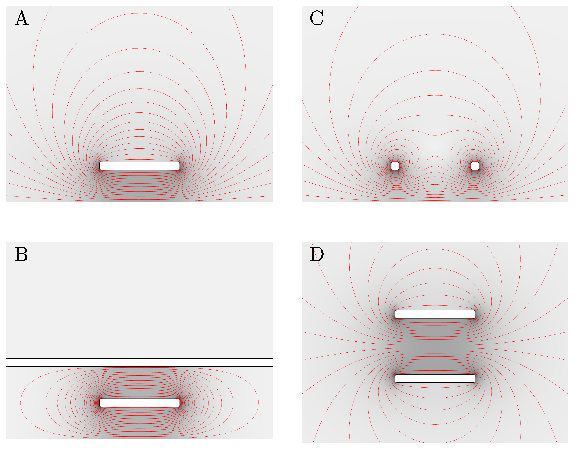
\includegraphics[width=\textwidth]{cross-sections}
	\end{center}
	\caption{Cross section of some typical planar transmission line geometries,
  		including magnetic field lines of the TEM mode. A: microstrip, B: stripline, C: microslot, D: parallel plate transmission line}
	\label{fig:cross-sections}
\end{figure}

\subsection{Characteristic Impedance and Transport
Characteristics}\label{characteristic-impedance-and-transport-characteristics}

For TEM modes, it is possible to attribute a current and a voltage
amplitude to the travelling wave by integrating along the electric /
magnetic field lines in the cross section. While the absolute voltage
and current amplitudes depend on the level of wave excitation, their
ratio (measured in Ohm) is a constant given purely by the cross section
geometry, and the dielectric and magnetic properties of the insulating
medium. This ratio is known as the characteristic impedance \m{Z_0} of
the wave guide. Coaxial cables are commonly designed for a
characteristic impedance of 50 Ohm.

\subsection{Theory of TEM Wave Modes}\label{theory-of-tem-wave-modes}

Maxwell's curl equations couple the magnetic field \m{\mathbf{H}} and
the electric field \m{\mathbf{E}}. If we assume a harmonic time
evolution of the fields with angular frequency \m{\omega}, they become
%
\begin{eqnarray}
\nabla \times \mathbf{H} &= j \omega \epsilon \mathbf{E} \\
\nabla \times \mathbf{E} &= - j\omega \mu \mathbf{H}
\end{eqnarray}
%
where \m{j=\sqrt{-1}} is the imaginary unit, and \m{\epsilon} and
\m{\mu} represent the electric permittivity and magnetic permeability of
the insulating medium, respectively. In order to analyse a TEM mode, we
assume the axis of the transmission line to be aligned with the z
direction. The two curl equations can be combined to the Helmholtz
equation
%
\begin{equation}
(\nabla^2+k^2) \mathbf{E}  =0,
\end{equation}
%
where \m{k=\omega\sqrt{\mu\epsilon}} is the wave number. If we assume a
harmonic dependence in the z direction of the two transverse components,
proportional to \m{e^{-j k z}}, it is easily shown that the transverse
components must satisfy Laplace's equation, i.e.,
%
\begin{equation}
\left(\frac{\partial^2}{\partial x^2}+ \frac{\partial^2}{\partial y^2}\right) E_{x,y} = 0.
\end{equation}

A similar argument leads to the same result for the transverse magnetic
field. The electric and magnetic field distribution in the cross section
of a transmission line are therefore solutions to Laplace's equation.
The fields satisfy the boundary conditions
\m{\mathbf{E} \cdot \mathbf{n}=0} and \m{\mathbf{H}\times \mathbf{n}=0},
where \m{\mathbf{n}} is the surface normal. It is useful to note that
the field distributions follow the same laws as in the case of
completely static fields. In particular, this means that the field
distribution inside a transmission line is
\textit{independent of the frequency}. Transmission lines are therefore
inherently broad-band devices, with no lower limit to the frequencies
they can carry. In theory, there is no upper limit for the propagation
of the TEM mode either; however, the excitation of TE and TM modes
complicates the situation at very high frequencies. For this reason,
coaxial transmission lines are only used up to frequencies of several
tens of GHz. In addition, dielectric losses in commonly used insulators
become intolerable at very high frequencies. 

\subsection{Modelling of TEM modes}\label{modelling-of-tem-modes}

Since the transverse electric and magnetic field distributions for TEM
modes are solutions of the two-dimensional Laplace equation, they are
easily computed for any geometry using a finite element or finite
difference approach. It should be noted that the electric field is
curl-free. Therefore, it can be represented as the gradient of an
electrostatic potential \m{\phi(x,y)}, which also satisfies the Laplace
equation. Computing the transverse field distribution therefore reduces
to a simple Dirichlet problem, where fixed potential values must be
attributed to the conductor surfaces:
%
\begin{equation}
\nabla^2 \phi(x,y)=0 \quad\text{on }B, \qquad \phi=V_{1,2,\dots}\quad\text{on } \partial B_{1,2,\dots}, 
\end{equation}
where $B$ denotes the dielectric cross section, and $\partial B_{1,2,\dots}$
represent the conductor surfaces, and $V_{1,2,\dots}$ are the electrical
surface potentials.
The electric field of a propagating TEM mode is then given by
\begin{equation}
	\mathbf{E}=e^{-\gamma z} \left(-\frac{\partial\phi}{\partial x}, -\frac{\partial\phi}{\partial x},0\right),
\end{equation}
where $\gamma=\alpha+j k$ is the propagation constant, which describes both
the oscillatory propagation of the wave in the z direction with wave
number \m{k} and its gradual attenuation with decay constant \m{\alpha}.
\footnote{It should be noted that the foregoing treatment is only strictly exact in the 
limit $\alpha \ll k$. However, for transmission lines composed of polymer
dielectrics and good conductors, this is almost always true to a 
good approximation.}

The magnetic field distribution
is easily found using the the curl equations:
\begin{equation}
		\mathbf{H}=e^{-\gamma z} \left(\frac{1}{\eta}-\frac{j\alpha}{\omega\mu} \right)\left(\frac{\partial\phi}{\partial x}, -\frac{\partial\phi}{\partial y},0\right),
\end{equation}
where the characteristic impedance of the medium $\eta$ is given by
\begin{equation}
	\eta=\sqrt{\frac{\mu}{\epsilon}}.
\end{equation}
Note that in the case of $\alpha=0$, the magnetic and the electric field are \textit{in phase},
whereas a positive attenuation constant $\alpha>0$ leads to the magnetic field phase lagging behind the electric field.
%
The time-averaged power transported by the TEM wave is given by real part the 
Poynting vector as
\begin{equation}
	\Re(\mathbf{S})=\frac{1}{2}\Re(\mathbf{E}\times\mathbf{H}^\ast) = p_t\,\hat{\mathbf{z}},
\end{equation}
where the cross-sectional density of power $p_t(x,y)$ is
\begin{equation}
	p_t(x,y)=\frac{e^{-2\alpha z}}{2\eta} \left[\left(\frac{\partial\phi}{\partial x}\right)^2+\left(\frac{\partial\phi}{\partial y}\right)^2\right].
\end{equation}
The relative power loss per unit length is therefore given by
\begin{equation}
	 \frac{1}{p_t}\frac{\partial p_t}{\partial z} = -2\alpha.
\end{equation}

At every cross section of
the transmission line, it is possible to compute the electrical
potential difference between the two conductors by a path integral 
between the condutcor surfaces
%
\begin{equation}
V(z) = \oint_1^2 \mathbf{E}(x,y,z)\cdot \mathrm{d}\mathbf{s},
\end{equation}
%
Similarly, the current flowing in the conductor can be obtained using
Ampere's law
%
\begin{equation}
I(z) = \oint \mathbf{H}(x,y,z)\cdot \mathrm{d}\mathbf{s},
\end{equation}
%
where the integration path in this case is a closed loop around the
conductor. 


It is easily shown that the voltage and current thus obtained
satisfy the equations
%
\begin{eqnarray}
\frac{\mathrm{d}^2 V}{\mathrm{d}z^2} = \gamma^2 V(z) \\
\frac{\mathrm{d}^2 I}{\mathrm{d}z^2} = \gamma^2 I(z).
\end{eqnarray}
%
These equations are useful to describe the behaviour of transmission
lines when integrated into electrical circuit networks. In general, they
can be solved by a superposition of two waves travelling in opposite
directions:
%
\begin{eqnarray}
V(z) = V_0^+ e^{-\gamma z} + V_0^- e^{\gamma z} \\ 
I(z) = I_0^+ e^{-\gamma z} + I_0^- e^{\gamma z}.
\end{eqnarray}

The ratio
%
\begin{equation}
Z_0 = \frac{V_0^+}{I_0^+} = \frac{V_0^-}{I_0^-}
\end{equation}
%
is known as the characteristic impedance of the transmission line. Its
value depends entirely on the geometry of the transmission line cross
section and on the the dielectric and magnetic properties of the
insulator.



\subsubsection{Losses in Transmission
Lines}\label{losses-in-transmission-lines}

There are two main contributions to the power losses in a transmission
line. On the one hand, there are dielectric losses due to the repeated
polarisation and depolarisation of the insulating medium. These are
proportional to the magnitude of the electric fields. The dielectric
properties of most insulator materials are only very weakly frequency
dependent; the dissipated power therefore tends to be proportional to
the frequency. The dielectric dissipation of a material can be expressed
by an imaginary component in its dielectric permittivity
\m{\epsilon=\epsilon' + i \epsilon''}. Often, the loss tangent, defined
as \m{\tan \delta = \epsilon''/\epsilon'} is used in order to characterise
the material. A second (and, in the present context, often
dominant) source of losses is the finite conductivity of the metallic surfaces.
A plane electromagnetic wave impinging on an imperfect
conductor penetrates into it only to a finite depth \m{\delta_s}, known as
the skin depth. This is because the tangential component of the magnetic
field at the boundary induces in the surface a current which cancels the
magnetic field deeper inside metal. Since this current is sustained
against a finite ohmic resistance, it leads to heating and therefore to
a loss of power from the electromagnetic wave. The dissipated power
depends linearly on the magnetic field at the surface of the conductor.
If the dimensions of the transmission line cross section are much larger
than the skin depth, it is possible to express the average dissipated power per
unit surface area as
%
\begin{equation}
P_\delta = \frac{1}{2}|H_\parallel|^2 R_s,
\end{equation}
%
where \m{R_s} is the surface resistance of the metal. It depends on the
material's conductance and the skin depth as
%
\begin{equation}
R_s = \frac{1}{\sigma \delta_s} = \sqrt{\frac{\omega\mu}{2\sigma}},
\end{equation}
%
where \m{\delta_s} is the skin depth, and \m{\sigma} represents the
conductivity. For pure Cu, \m{\sigma=5.9\cdot 10^7}S/m, which translates
into a surface resistance of about 10 m\m{\Omega} at 100 MHz, and about
35 m\m{\Omega} at 1 GHz. The losses lead to a gradual attenuation of a
travelling TEM mode, as reflected in the real part of the propagation
constant \m{\gamma}. The conductive and dielectric losses are additive,
such that we can write
%
\begin{equation}
\alpha = \alpha_d + \alpha_c.
\end{equation}

In the following, we examine some planar transmission line geometries,
and the relationship between their geometry, characteristic impedance,
and attenuation constants.

\subsection{Magnetic Fields and Losses in Transmission Lines,
Striplines, Microstrips and
Microslots}

The magnetic and electric field distributions of the TEM mode in some
planar transmission line geometries are shown in Fig XXX. Fig XXa shows
a stripline, symmetrically bounded between two ground planes. The
magnetic field lines encircle the central conductor, producing two areas
of very high field homogeneity which can be used as sample locations for
NMR spectroscopy. The stripline, shown in Fig. XXb, exhibits a similar
field geometry. However, since there is only a single ground plane, the
magnetic and electric fields penetrate into the free space above. This
is less pronounced in practice than in the idealised computation shown
here, since the dielectric constant of the insulator means that the
electric field remains partially captured inside it. Nonetheless, the
open geometry can lead to radiation losses, which must be kept to a
minimum by external shielding. Fig. XXXc shows a microslot line. In this
case, there are two independent conductors, which can in principle carry
different electrical potentials. This geometry is therefore capable of
supporting more than one TEM mode. However, in the present context, only
the common mode shown in Fig. XXXc is of interest. Compared to the
similar microstrip geometry, the magnetic field is concentrated in the
space immediate above the pair of conductors.

\subsubsection{Transmission Line
Resonators}\label{transmission-line-resonators}

\begin{itemize}
\item
  Dimensions and eigenfrequencies
\item
  Q factor and sensitivity
\item
\end{itemize}
